\appendix

\section{Metodų skirtų daugiamačių duomenų indeksavimui apžvalga}
\label{app:multidimensionalIndexing}
\begin{figure}[H]
\begin{center}
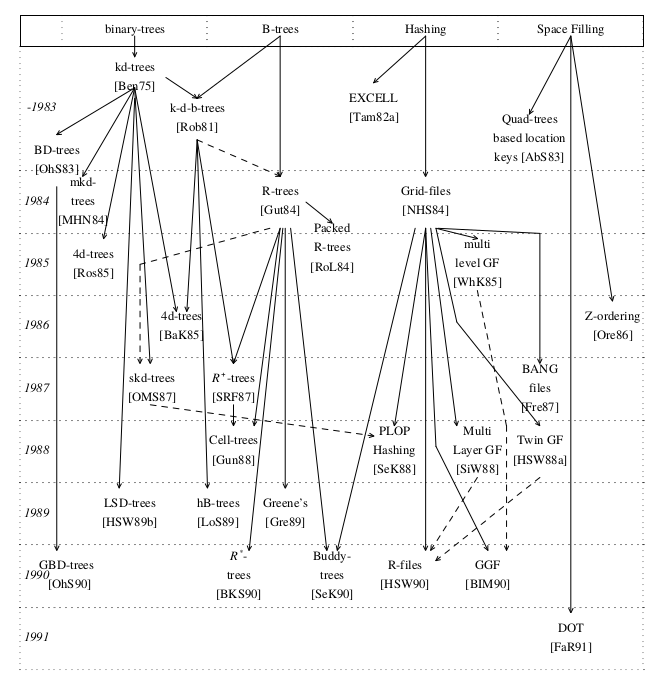
\includegraphics[width=\textwidth]{img/MultidimensionalDataIndexing.png}
\caption{\cite{bader2012space} pateikiama metodų, skirtų daugiamačių duomenų indeksavimui, schema}
\end{center}
\end{figure}

\section{Įvairių užklausų pavyzdžiai}

\label{app:pointQuery}
\begin{figure}[H]
\begin{center}
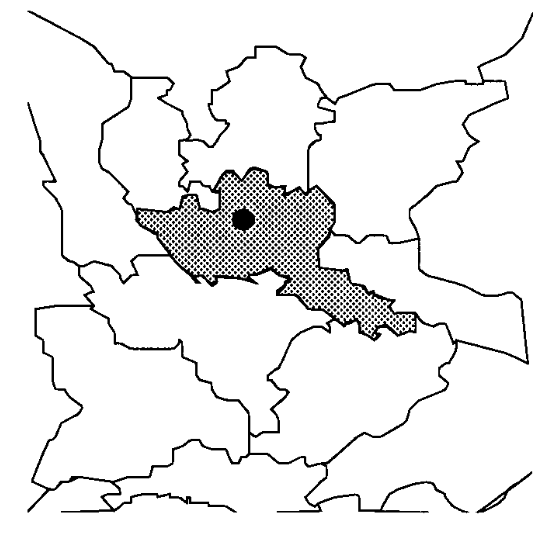
\includegraphics[width=0.4\textwidth]{img/PointQuery.png}
\caption{Taško užklausos pavyzdys}
\end{center}
\end{figure}

\label{app:windowQuery}
\begin{figure}[H]
\begin{center}
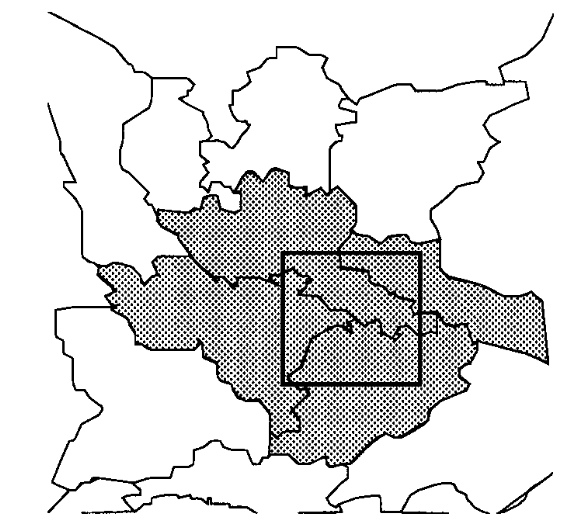
\includegraphics[width=0.4\textwidth]{img/WindowQuery.png}
\caption{Lango užklausos pavyzdys}
\end{center}
\end{figure}

\label{app:enclosureQuery}
\begin{figure}[H]
\begin{center}
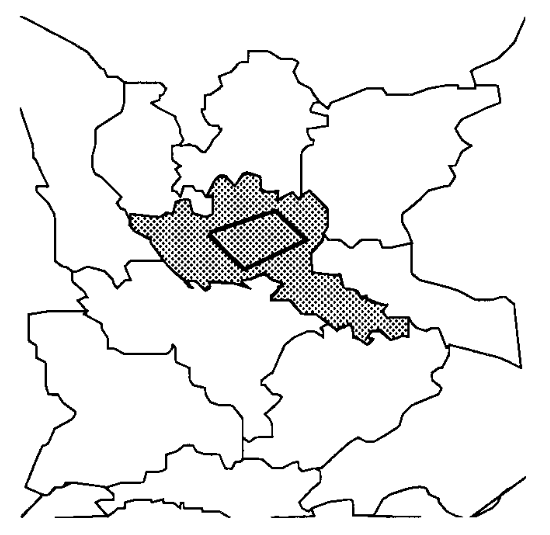
\includegraphics[width=0.4\textwidth]{img/EnclosureQuery.png}
\caption{Apgaubiančiosios užklausos pavyzdys}
\end{center}
\end{figure}

\label{app:intersectionQuery}
\begin{figure}[H]
\begin{center}
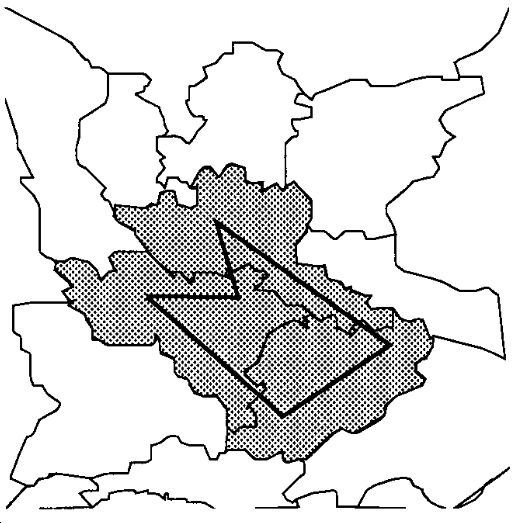
\includegraphics[width=0.4\textwidth]{img/IntersectionQuery.png}
\caption{Regiono užklausos pavyzdys}
\end{center}
\end{figure}

\label{app:containmentQuery}
\begin{figure}[H]
\begin{center}
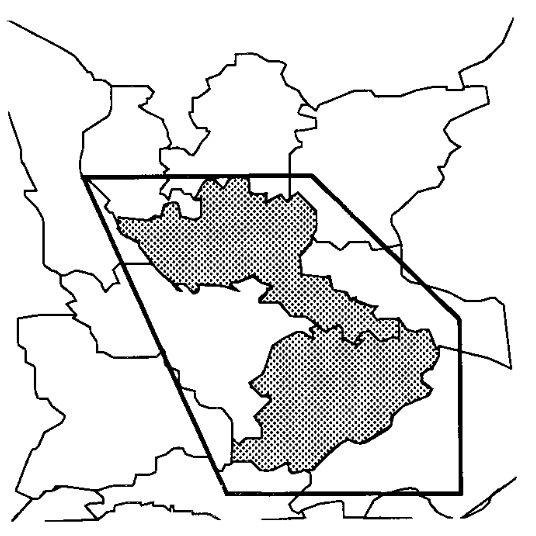
\includegraphics[width=0.4\textwidth]{img/ContainmentQuery.png}
\caption{Pilno regiono užklausos pavyzdys}
\end{center}
\end{figure}

\label{app:adjacencyQuery}
\begin{figure}[H]
\begin{center}
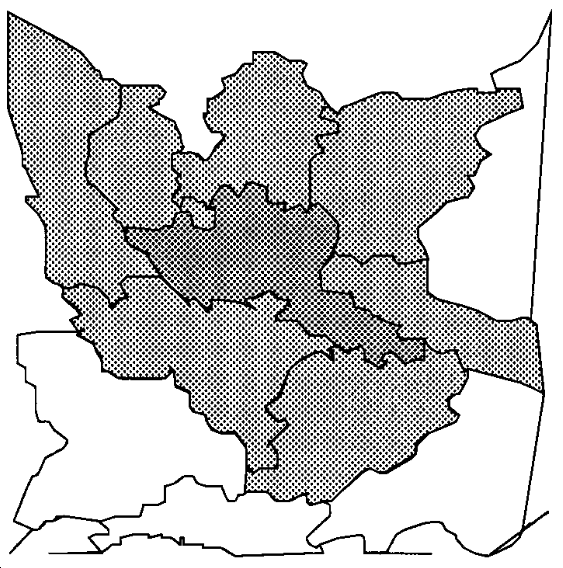
\includegraphics[width=0.4\textwidth]{img/AdjacencyQuery.png}
\caption{Kaimynų užklausos pavyzdys}
\end{center}
\end{figure}







